\documentclass[10pt,letterpaper]{article}
\usepackage[margin=0.55in]{geometry}
\usepackage{amsmath,graphicx,booktabs,caption}
\captionsetup{font=footnotesize,labelfont=bf,skip=3pt}
\pagestyle{empty}
\begin{document}
\begin{center}{\large\bfseries Your universe at the best fit: thin constant-density shell hugging our visible sphere plus a CoE core}\end{center}
\vspace{-8pt}
\begin{figure}[h]\centering
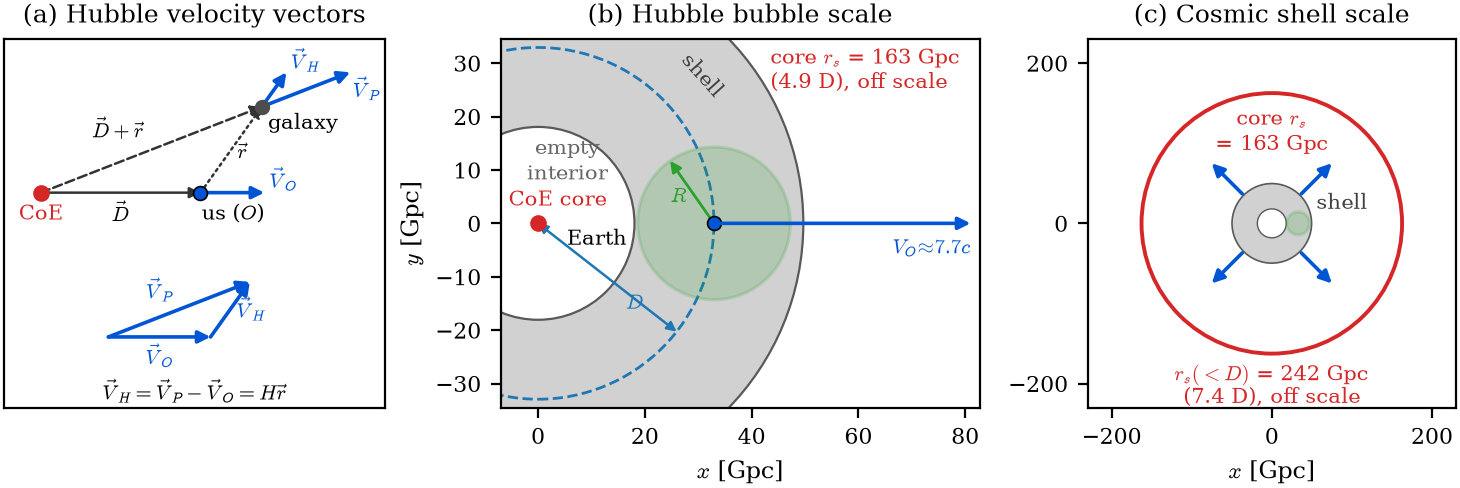
\includegraphics[width=\textwidth]{universe_thin_drawing.png}
\caption{Three scales, left to right, at the best fit with $\Omega_s$ free; (b) and (c) are to scale in Gpc with equal axes. (a) Hubble velocity vectors. In a Sedov--Taylor blast wave (Taylor 1950; Sedov 1959) the velocity grows in proportion to distance from the centre, $\vec V = k\,\times$(position from the CoE) for some constant $k$. So we, at position $\vec D$, move with $\vec V_O = k\vec D$, and a galaxy at $\vec D+\vec r$ moves with $\vec V_P = k(\vec D+\vec r)$. Their relative velocity is $\vec V_H = \vec V_P-\vec V_O = k\vec r$, which is Hubble's law, so $k = H$. It depends only on the separation $\vec r$, so the CoE drops out and every observer sees the same isotropic Hubble flow. (b) Hubble bubble: the grey shell has constant density $\Omega_s=1.01$ (about 20 times the ordinary-matter density) from $R_{\rm in}=D-R=79.4$ to $R_{\rm out}=D+R=108.0$~Gpc, the interior is empty apart from the CoE core, the dashed circle of radius $D=93.7$~Gpc runs through Earth, and the green disc is the vision sphere of radius $R=14.3$~Gpc. The red arc is the core's own Schwarzschild radius $r_s=2GM/c^2=119$~Gpc ($1.27\,D$), already beyond Earth. Earth moves outward along $+x$, the anti-CoE direction $\ell_0=12.8^\circ$ (sky directions are Galactic longitude, $\theta=\ell-\ell_0$). (c) Cosmic shell: the shell, the core's $r_s$ and Earth's turnaround radius (991~Gpc, $10.6\,D$); the $r_s$ of all mass inside $D$ is 17{,}907~Gpc ($191\,D$), off scale. Blue arrows are velocities in all panels. In this Newtonian model Earth moves outward at $V_O=19.7\,c$, is bound ($(V_O/v_{\rm esc})^2=0.90$) and turns around after 55 ages; the mass inside has $r_s\approx42{,}000$~Gpc, so turnaround lies inside $r_s$ and in general relativity the region would recollapse.}
\end{figure}
\vspace{-10pt}
\noindent\begin{minipage}[t]{0.50\textwidth}\vspace{0pt}\centering
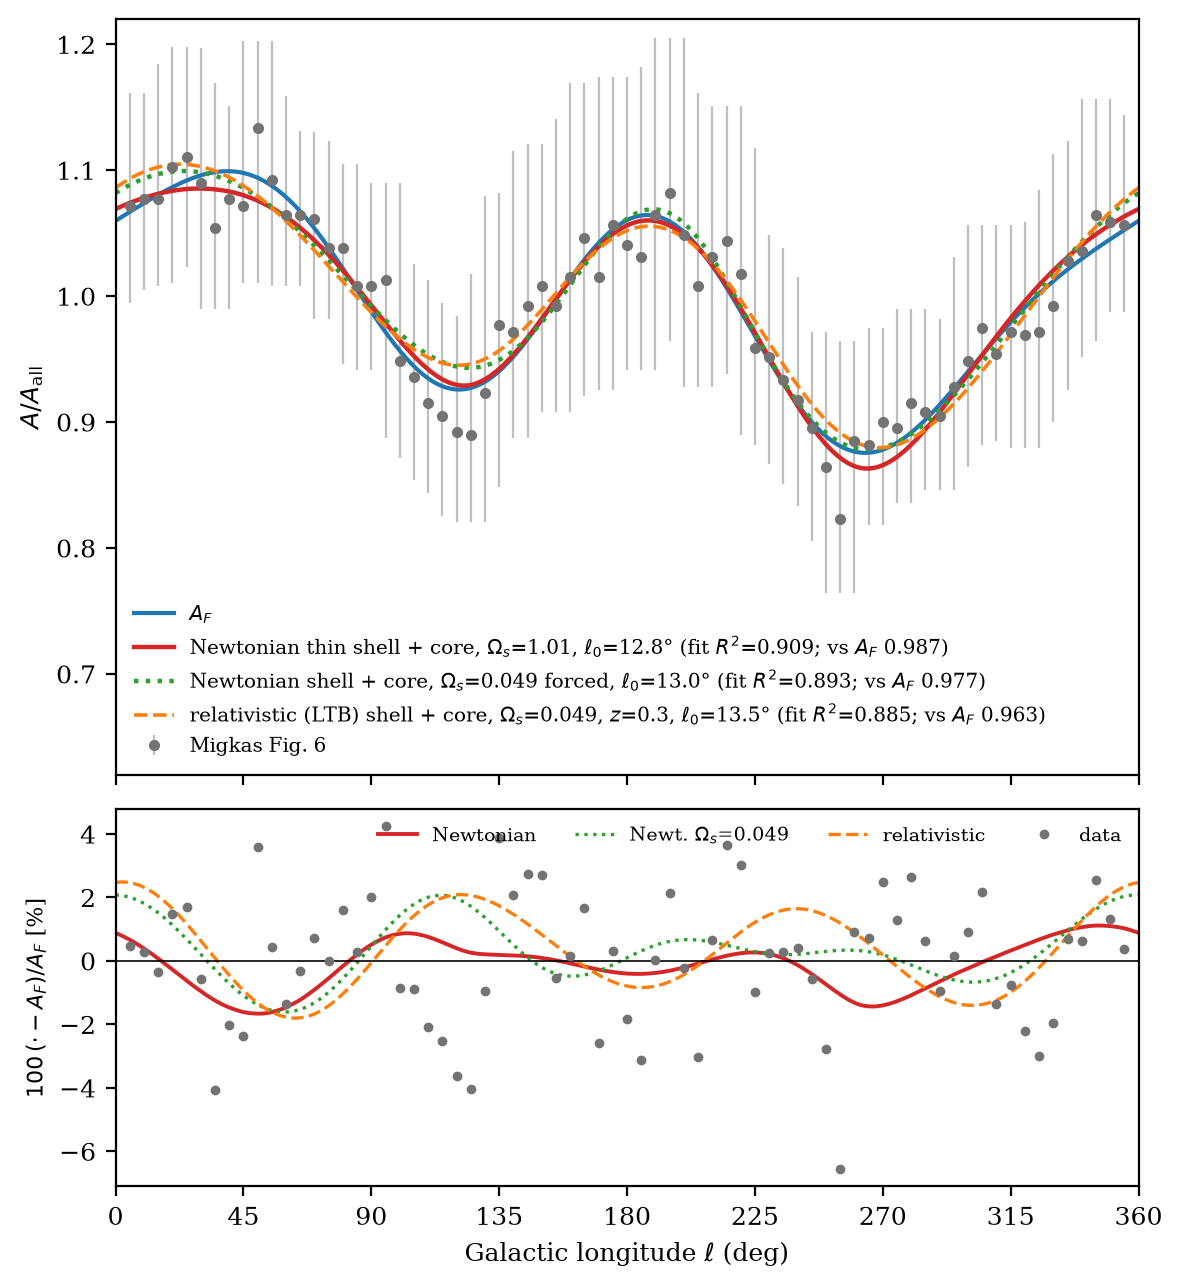
\includegraphics[width=\textwidth]{universe_thin_Achart.png}
\captionof{figure}{Migkas points with error bars, $A_F$, and your model A for the thin shell with a core, normalised to the sky mean. Solid: shell density free ($\Omega_s=1.01$). Dashed: the same model with the shell density fixed at 0.05 of critical, about the density of ordinary matter. The lower panel shows data and models as percent differences from $A_F$. The sources spend almost all their history coasting through the empty interior, where only the CoE core pulls on them, so the core sets the pattern ($\ell_0\approx13^\circ$).}
\end{minipage}\hfill
\begin{minipage}[t]{0.48\textwidth}\vspace{0pt}\centering\scriptsize\setlength{\tabcolsep}{2.2pt}\renewcommand{\arraystretch}{0.93}
\captionof{table}{Best-fit values in your sheet's cells: integrated model ($G$ real, from $0.01\,t_0$, fixed in space, $H_0=70$), shell from $D-R$ to $D+R$, $\ell_0$ free. B27 is all gravitating mass inside $D$. The second column is the same geometry with the shell at ordinary-matter density ($\Omega_s=0.05$).}
\begin{tabular}{llll}\toprule
Cell & Quantity & $\Omega_s$ free & $\Omega_s=0.05$\\\midrule
C23 & $D/R$ & 6.554 & 3.474\\
D23 & $L_c/D$ (core size) & 0.0050 (bound) & 0.0050 (bound)\\
B29 & $R$ & $4.4127\times10^{23}$ km & same\\
 &  & (14.30 Gpc) & \\
B28 & $D$ & $2.8919\times10^{24}$ km & $1.5331\times10^{24}$ km\\
 &  & (93.72 Gpc) & (49.69 Gpc)\\
B30 & $L_c$ & $1.45\times10^{22}$ km & $7.67\times10^{21}$ km\\
 &  & (0.469 Gpc) & (0.248 Gpc)\\
B27 & $M(<D)$, total & $3.720\times10^{56}$ kg & $4.676\times10^{54}$ kg\\
 &  & $1.87\times10^{26}$ $M_\odot$ & $2.35\times10^{24}$ $M_\odot$\\
 & $M_c$, core & $2.47\times10^{54}$ kg & $2.38\times10^{53}$ kg\\
 & $M_c/M_{\rm crit}(D)$ & 0.00265 & 0.00172\\
 & $M_{\rm shell}(<D)$ & $3.70\times10^{56}$ kg & $4.44\times10^{54}$ kg\\
 & $M_{\rm hole}$ & $5.74\times10^{56}$ kg & $2.51\times10^{54}$ kg\\
BA57 & Amp & $-$0.1240 & $-$0.0622\\
BA59 & $\varphi$ & 1.264 rad & 0.933 rad\\
 & $\ell_0$ & 12.82$^\circ$ & 13.25$^\circ$\\
\midrule
 & $\Omega_s$ & 1.012 & 0.05 (ordinary matter)\\
 & $\rho_s$ & $9.32\times10^{-27}$ kg\,m$^{-3}$ & $4.60\times10^{-28}$ kg\,m$^{-3}$\\
 & $R_{\rm in}=D-R$ & 79.4 Gpc & 35.4 Gpc\\
 & $R_{\rm out}=D+R$ & 108.0 Gpc & 64.0 Gpc\\
 & $r_s$, core & 119 Gpc (1.27\,$D$) & 11.5 Gpc (0.23\,$D$)\\
 & $r_s$, all mass $<D$ & 17{,}907 Gpc (191\,$D$) & 225 Gpc (4.5\,$D$)\\
\midrule
 & $(V_O/v_{\rm esc})^2$ & 0.901 (bound) & 10.56 (unbound)\\
 & Turnaround radius & 991 Gpc (10.6\,$D$) & none\\
 & Age $t_0$ & 13.8 Gyr & 13.9 Gyr\\
 & $\delta$ across sphere & 0 & 0\\
 & fit $R^2$ vs Migkas & 0.909 & 0.893\\
 & fit $R^2$ vs $A_F$ & 0.987 & 0.977\\
\bottomrule
\end{tabular}
\end{minipage}
\par\vspace{6pt}\noindent{\scriptsize\textbf{References.} Taylor, G.~I. 1950, Proc.\ R.\ Soc.\ Lond.\ A, 201, 159. Sedov, L.~I. 1959, Similarity and Dimensional Methods in Mechanics (New York: Academic Press).\par}
\end{document}
